\documentclass{book}
%%%%%%%%%%% PACKAGES %%%%%%%%%%%
% For margins
\usepackage[margin=0.8in,right=3cm]{geometry}

% For picture includes
\usepackage{graphicx}

% Used to set option H in figures
\usepackage{float}

% To wrap figures with text
\usepackage{wrapfig}

% URL in references
\usepackage{url}

% For code snippets
\usepackage{listings}

% For figure placing
\usepackage{float}

%For fancy mathmode stuff (mathbb etc)
\usepackage{amsfonts}


%For useful math stuff like cases, align* etc
\usepackage{amsmath}

% For todos
\usepackage[colorinlistoftodos]{todonotes}

% For subfigures and captions
\usepackage{subfigure}

% For new line instead of para indents
\usepackage[parfill]{parskip}

% Todo
\usepackage{todonotes}

% To do nested enumerations
\usepackage{enumitem}

\usepackage{verbatim}

% Formatting paragraphs as sections
\usepackage{titlesec}
\setcounter{secnumdepth}{4}
\titleformat{\paragraph}
{\normalfont\normalsize\bfseries}{\theparagraph}{1em}{}
\titlespacing*{\paragraph}
{0pt}{3.25ex plus 1ex minus .2ex}{1.5ex plus .2ex}



\title{Squat - A Computer Vision Driven Training Aid}
\author{Jack Stevenson}

\lstset{tabsize=2}
\lstdefinestyle{javastyle}{
  belowcaptionskip=1\baselineskip,
  breaklines=true,
  language=Java,
  showstringspaces=false,
  basicstyle=\ttfamily,
  keywordstyle=\bfseries\color{blue},
  commentstyle=\itshape\color{green!40!black},
  identifierstyle=\color{blue!40!black},
  stringstyle=\color{red},
}

\newenvironment{centersections}
{\titleformat{\chapter}[block]{\Large\bfseries\filcenter}{}{1em}{}}
{\titleformat{\chapter}[block]{\Large\bfseries}{}{1em}{}}

\raggedbottom

\begin{document}
\begin{titlepage}
\begin{center}

% Upper part of the page. The '~' is needed because \\
% only works if a paragraph has started.

\includegraphics[width=0.15\textwidth]{title/images/ImperialCrest}~\\[1cm]

\textsc{\LARGE Imperial College London}\\[1.5cm]

\textsc{\Large Final year project}\\[0.5cm]

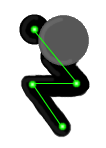
\includegraphics[width=0.10\textwidth]{title/images/squatslim}~\\

% Title
\noindent\rule{12cm}{0.6pt} \\
{ \huge \bfseries Squat! \\ A Computer Vision Driven Training Aid \\[0.4cm] }
\noindent\rule{12cm}{0.6pt} \\[1cm]

% Author and supervisor
\begin{minipage}{0.4\textwidth}
\begin{flushleft} \large
\emph{Author:}\\
Jack \textsc{Stevenson}
\end{flushleft}
\end{minipage}
\begin{minipage}{0.4\textwidth}
\begin{flushright} \large
\emph{Supervisor:} \\
Prof.~Andrew \textsc{Davision}
\end{flushright}
\end{minipage}

\vfill

% Bottom of the page
{\large \today}

\end{center}
\end{titlepage}
\pagebreak

\large

\begin{centersections}
\section*{Abstract}

Squats are a common exercise used by both athletes in their training and amateurs lifting weights recreationally. As a reasonably advanced compound movement, squats can often be performed incorrectly, leading to an ineffective training programme and potentially serious injury. This project offers a solution to this problem- an application called \emph{Squat!}. \emph{Squat!} is a real-time squat tracking and analysis application, which employs computer vision to examine a user's squat technique whilst they are performing the lift, offering immediate feedback. In this project a non-intrusive, marker-less algorithm to track and analyse a lifter's pose using a monocular camera has been developed and implemented to run in real-time on a mobile device. The result of this project is an intuitive and accurate application for use as a training aid, enabling users to improve the safety and effectiveness of their squats.
\pagebreak
\section*{Acknowledgements}

Firstly I would like to thank my supervisor, Professor Andrew Davison, for supporting me throughout this project. His feedback, advice and suggestions were all incredibly helpful in developing the algorithm and keeping to schedule.

I would also like to thank Professor Duncan Gillies, my second marker, for his support during the initial stages of the project.

Thank you to Tom Wilding, Greg Pye and Harry Stevenson for testing the application in the evaluation stage of the project, and offering feedback and ideas to improve the application.
\end{centersections}

\pagebreak
\tableofcontents

\pagebreak
\section{Introduction}
This is an example of splitting sections into folders.

\subsubsection{Subsection}
This is a subsection in the intro directory. This references Google\cite{google}.
\pagebreak
\section{Background}

%Background (10- 20 pages).  This should form the bulk of the interim report. You should consider that your objective here is to produce a near final version of the background section, as it will appear in your final report.  All of this material should be re-usable, so it is worth getting it right at this stage of the project.  The details of what to include can be found in the Project Report guidelines.

%The background section of the report should set the project into context by relating it to existing published work which you read at the start of the project when your approach and methods were being considered. There are usually many ways of solving a given problem, and you shouldn't just pick one at random. Describe and evaluate as many alternative approaches as possible. The published work may be in the form of research papers, articles, text books, technical manuals, or even existing software or hardware of which you have had hands-on experience. Your must acknowledge the sources of your inspiration. You are expected to have seen and thought about other people's ideas; your contribution will be putting them into practice in some other context. However, avoid plagiarism: if you take another person's work as your own and do not cite your sources of information/inspiration you are being dishonest; in other words you are cheating. When referring to other pieces of work, cite the sources where they are referred to or used, rather than just listing them at the end. Make sure you read and digest the Department's plagiarism document .

%In writing the Background chapter you must demonstrate your capability of analysis, synthesis and critical judgement. Analysis is shown by explaining how the proposed solution operates in your own words as well as its benefits and consequences. Synthesis is shown through the organisation of your Related Work section and through identifying and generalising common aspects across different solutions. Critical judgement is shown by discussing the limitations of the solutions proposed both in terms of their disadvantages and limits of applicability.

\subsection{A Stereo Approach}

A large amount of research has been done in the use of stereo cameras and 3D sensors for skeletal tracking. Much of this arose from the introduction of Microsoft's Kinect\cite{kinect} sensor which brought affordable and reliable depth perception to the general public.

\subsubsection{Kinect}

Jamie Shotton et al developed an algorithm\cite{shottonkinect} for human pose detection (that is the three-dimensional positions of body joints) which uses a Randomised Decision Forest trained on an extremely large data set of a wide variety of poses. This machine learning approach is used in the Kinect tracking system, and has the advantage of being both robust and computationally inexpensive to classify a new image. This is due to the algorithm reducing the detection into a per-pixel classification problem. Another advantage of this method is that it does not rely on temporal information (or previous frames) as pose estimation can be performed on a standalone frame.

However this machine learning approach may not be feasible in the scope of this project. There is not enough time available to collect the data required to train a machine learner such as this to recognise body pose. Shotton's results showed that in order to effectively detect a human pose, his system required training on at least 100,000 images\cite{shottonkinect}.
\subsubsection{Captury}

A company known as Captury\cite{captury} have constructed a method for robust motion capture using a stereo camera. In their paper `On-set Performance Capture of Multiple Actors With A Stereo Camera'\cite{capturystereopaper} they describe a method that ``employs appearance cues, scene flow, pose reconstruction results from previous frames, and stereo coherence to reliably segment out actors in front of general backgrounds.''. This method has been shown to be highly robust, and Captury have provided a video\cite{capturyvideo} to demonstrate this. Not only does their method track the skeleton, it also performs a further step to map a full three dimensional body to the video, for full motion capture.

Although immensely accurate, Captury's process requires a large amount of computation, in the order of minutes per frame. This means that use of an algorithm following their pipeline would not be able to achieve real-time feedback.

\subsubsection{Applied to this Project}

Unfortunately, despite the wide array of tools and libraries available for skeletal tracking with a 3D sensor or stereo camera, it would be infeasible to take a device like a Kinect hooked up to a computer into a gym. Perhaps if the goal were to have the system set up at powerlifting competitions, or pre-installed at gyms, this method would be more reasonable. However as a personal training aid, the device must be portable.

Another alternative option would be to develop an application for a smartphone with a stereo camera. Smartphones such as the LG Optimus 3D\cite{lgoptimus} provide such a camera. However these phones are not currently in wide use and would severely narrow the audience for this application.

For these reasons it has been chosen to employ a monocular approach. This will make foreground segmentation more challenging and so it has been decided to narrow the scope of the project to a known camera angle.


\section{Human Models}

A key part of my project will be the creation of a reliable human model to map to each frame, so that it mimics the pose of the lifter. In this section potential model options for use in this project will be considered.

\subsubsection{A Cardboard Model}

A possible representation is a so called ``carboard model'', which is a set of interconnected planar patches used to represent human limbs. This is used in `Cardboard People: A Parameterized Model of Articulated Image Motion'\cite{cardboardpeople}, where S. Ju et al tracked a walking movement in two dimensions using two body parts - the thigh and the calf. These articulated components were governed by their `translation' and `curl' (that is rotation) in a side view of the walk. For more robust modelling from other camera angles, components could be governed by their `divergence', `deformation', `yaw' and `pitch'. The culmination of these parameters defines each cardboard segment's location in two-dimensional space, but compensates for three-dimensional movement of the subject. Figure~\ref{fig:cardboardmodel} shows an example model and the effects of adjustments of these parameters.

\begin{figure}[H]
    \centering
    \subfigure[A cardboard model]{
            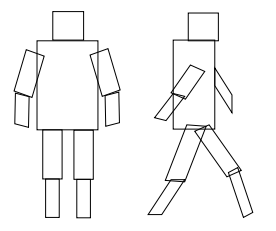
\includegraphics[height=6cm]{background/images/cardboard}
    }
    \subfigure[Parameters governing position of a cardboard segment]{
            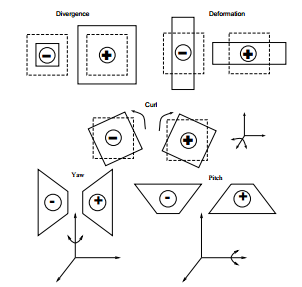
\includegraphics[height=6cm]{background/images/cardboard2}
    }
\caption{The cardboard model used by S. Ju et al\cite{cardboardpeople}}
\label{fig:cardboardmodel}
\end{figure}

Other similar primitive shape representations such as cylinders, ellipsoids and cones are often used\cite{cvmocapsurvey}.
\subsubsection{Stick Figure Model}

Motion capture of human walking has been carried out in `Lower Limb Kinematics of Human Walking with the Medial Axis Transformation'\cite{stickfigure}, where instead of a fleshed out model like the cardboard model, A. Bharatkumar et al used a stick figure to represent the human body. In this paper they concluded that ``It is easier to track the segment angles of the thigh and leg than the actual positions of the joints''. This makes mapping much simpler than that of the cardboard model, as there are far fewer parameters to optimise. Although they did not add explicit constraints to the model in their paper, it would be easy to add such constraints to ensure a better fit of the model to the frame. Figure~\ref{fig:stickfiguremodel} shows a full three-dimensional stick figure model, and a two-dimensional model of the thigh and calf.

\begin{figure}[H]
    \centering
    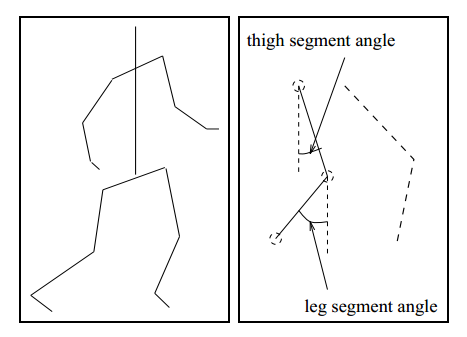
\includegraphics[height=6cm]{background/images/stickfigure}

	\caption{The stick figure model used by A. Bharatkumar et al\cite{stickfigure}}
	\label{fig:stickfiguremodel}
\end{figure}
\subsubsection{A Three-Dimensional Model}

As well as models constructed from primitive two-dimensional shapes, we can extend these models into three dimensions. Some solutions are simple expansions of these primitives into their three-dimensional counter parts, but others are more intricate. M. Yamamoto et al used Computer Aided Design to develop a model constructed of conical cylinders and cuboids\cite{cadmodel}. Another example of this is shown in Figure~\ref{fig:3dmodelajd} where a range of three-dimensional shapes are mapped to a human figure by J. Deutscher et al.

\begin{figure}[H]
    \centering
    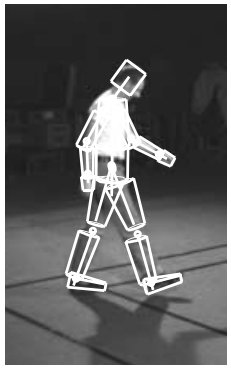
\includegraphics[height=6cm]{background/images/3dpolygon}

	\caption{A model constructed of three-dimensional primitive shapes\cite{stickfigure}}
	\label{fig:3dmodelajd}
\end{figure}

Some have used more advanced techniques to construct a customised model to be used to track a known person. C. Wu et al performed a three-dimensional scan of the subjects to generate a textured model of each person to be tracked\cite{capturystereopaper}. Several others have used similar techniques, creating a more `life like' model of a human. This has advantages in being able to fit the subject more accurately, but requires an additional step to create the model of a new subject prior to tracking them. Figure~\ref{fig:3dtexturedmodel} shows an example of a model generated in this way and mapped to a frame of video.

\begin{figure}[H]
    \centering
    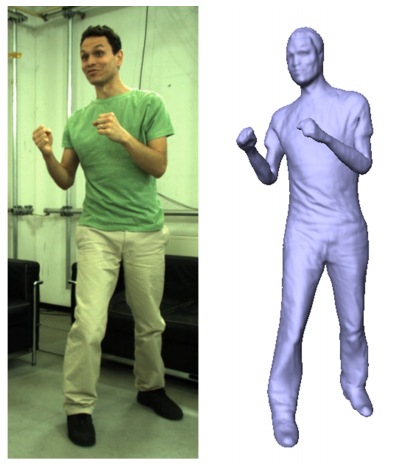
\includegraphics[height=6cm]{background/images/3dtexture}

	\caption{A more advanced model, specific to an individual subject\cite{capturystereopaper}}
	\label{fig:3dtexturedmodel}
\end{figure}
\subsubsection{Applied to this Project}

This project will be using a monocular camera. This does not necessarily mean that the mapping of a three dimensional model to a two dimensional frame is not impossible, but is more computationally challenging. In the case of squatting, we can extract all required data to determine the validity of a lift from a two dimensional model of the side view. The only information that we would miss with a two dimensional model is one related to the safety of the lifts: the position of the knees from a front view, to make sure that they do not buckle in towards each other. This is an acceptable compromise, being only a single measure out of many.

The camera will be in a known location relative to the human subject and the movements are well defined, which makes a two dimensional model feasible. As it will provide us with enough data to determine the validity and to measure the majority of safety criteria of the lift, I have opted to use a two dimensional model for this project.

This two dimensional model will likely be based on the cardboard model, using two dimensional shapes that best fit the human subject. Their positions should not individually be defined by their position, rotation, yaw etc, but should be defined by the relative rotations at joints. This will reduce the degrees of freedom of the model, allowing for faster optimisation. It will also more accurately represent a human and the human limits of joint movement can be used to constrain the optimisation problem.
\pagebreak
\chapter{Squat Technique}

In order to ensure that the application gives appropriate feedback, it is important to discern the factors that make a squat safe and correct.

Mark Rippetoe is a well established strength coach, and has published a book entitled Starting Strength\cite{startingstrength}. This book contains detailed information regarding the biomechanics of a squat. In this project, Rippetoe's work is used as the basis for a safe squat. There are a wide range of opinions on what makes a squat safe, and no official standard has been established, however Rippetoe's work is backed by biomechanical studies and has been proved safe and effective over his years of coaching athletes. In this section the most important factors affecting the safety and optimality of a squat are discussed in turn.

\section{Depth}

One of Rippetoe's primary factors that contribute to the safety of a squat is its depth. He explains:

\begin{quote}
\emph{The squat, when performed correctly, is not only the safest leg exercise for the knees, it produces a more stable knee than any other leg exercise. The important part of the last statement is the `when performed correctly' qualifier. Correctly is deep, with hips dropping below level with the 
top of the patella.}
\end{quote}

He continues to describe the way in which a squat that does not reach sufficient depth does not stress the glutes, adductors and hamstrings, whilst it does stress the knees, resulting in an \emph{`unbalanced strain on the prepatellar area'}.

Therefore it is important that the application takes depth into account when providing feedback on the safety of a squat.

\section{Weight Distribution}

Rippetoe explains that the lifter's hips can only be used correctly with the right back angle. He elaborates that the key factor to producing the correct back angle is to ensure that the bar is directly vertical to the middle of the foot:

\begin{figure}[H]
    \centering
	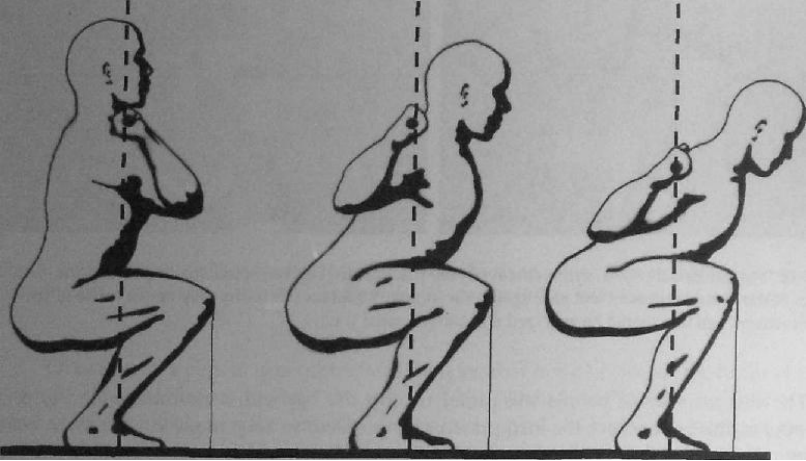
\includegraphics[height=7cm]{squat/images/rippetoe_weight_distro}
\caption{Squat weight distribution}
\label{fig:rippetoe_weight}
\end{figure}

\begin{quote}
\emph{Bar position ultimately determines back angle, as seen in this comparison of the front squat, the high-bar squat, and the low-bar squat.[\ref{fig:rippetoe_weight}] Note that the bar remains balanced over the mid-foot in each case, and this requires that the back angle accommodate the bar position.}
\end{quote}

The application should ensure that the bar is directly vertical to the foot throughout the lift.

\section{Back Angle and Knee Position}

Following on from this, there are also safety limits in the back angle and knee position. If the back angle is too close to horizontal or becomes rounded during the squat, it puts unnecessary strain on the lower back. If the back is too upright, the knees are pushed too far forward which causes strain on the patella. Rippetoe explains the detrimental effects of poor knee position:

\begin{quote}
\emph{Letting the knees travel forward at the bottom of the squat is both inefficient for posterior chain involvement and detrimental to the health of the hip flexor tendons.}
\end{quote}

He also explains the two most common problems with knee position in squats:

\begin{quote}
\emph{By far, the two most common knees errors are 1.) knees in too much and 2.) knees too far forward, either early in the descent or at the bottom.}
\end{quote}

Sadly due to the fixed position of the camera, the first error of knees buckling in towards each other cannot be addressed by the application. However this can be easily observed by the lifter when squatting in front of a mirror. The second error is straightforward to measure from a side view.

Rippetoe defines a good knee position:

\begin{quote}
\emph{Depending on your femur/tibia/trunk dimensions, your knee could be anywhere from directly above your toes to three or four inches in front of them.}
\end{quote}

The application should ensure both that the back angle is not too horizontal or vertical, and that the knees do not go too far in front of the toes.

\section{Knee and Hip Flexion}

Rippetoe also mentions the rate of relative knee and hip flexion as an important factor affecting the squat. When the angle of the knee increases at a faster rate than that of the hip in the upward stage of the squat, load is shifted to the quadriceps and away from the posterior kinetic chain (the glutes and hamstrings). This loads the spine and can open risk to injury.

This principle is shown in Starting Strength in figure~\ref{fig:rippetoe_flexion}.

\begin{figure}[H]
    \centering
	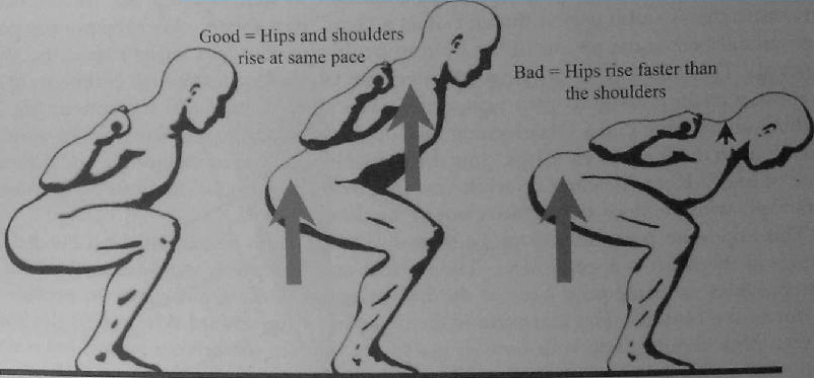
\includegraphics[height=6cm]{squat/images/rippetoe_knee_hip_flexion}
\caption{Relationship between the rate of change of the knee and hip angles}
\label{fig:rippetoe_flexion}
\end{figure}

The application should measure the rate of change of the hip and knee angles relative to one another and should penalise the lifter should the knee angle increase faster than the hip angle.

\section{Competition Rules}

The International Powerlifting Federation rules\cite{ipf} agree with Rippetoe's views on squat depth - a squat is only considered valid if the lifter descends to a point at which the hip joint is lower than the top of the knees.

The rules dictate that a squat is completed when the knees are locked and the lifter is upright. This state is known as `lockout'. The application must check that the lifter completed the full movement in order to count the squat as valid.

Another International Powerlifting Federation rule is that there should be no downward movement during the ascent stage of the squat. To have the application recognise this rule, there are two options. Either to penalise downward movement detected after starting an ascension and before locking out, or to treat any downward movement as the beginning of a new repetition. The second option allows for better segmentation of repetitions, counting squats that are not performed with the full range of motion as individual repetitions whilst penalising them appropriately for not including a lockout. The first option would only count repetitions that were fully locked out, giving a poor user experience to lifters that do not complete all of their squats successfully.
\pagebreak
\section{Core Algorithm}

In this section I will describe the algorithm that I have developed to solve the problem of real-time squat tracking and analysis.

\subsection{Detection}

Detection is the first component of the algorithm. This component allows the lifter to be located in the scene automatically and the model to be scaled to fit the lifter. Detection can be broken down into four main stages.

\subsubsection{Ensure Camera and Surroundings are Stationary}
Detection starts after ensuring that the camera is still and there is little or no movement in the background. This is done using OpenCV's \texttt{Background SubtractorMOG}. This background subtractor is based on the work of P. KaewTraKulPong et al\cite{backgroundsubmog}. It can be provided with a learning rate and history as parameters, which determine how quickly new pixels in the foreground are adopted as part of the background model. During this initial stage, a low history and high learning rate is used, meaning that when the frame contains no motion, the entire scene quickly becomes background. The percentage of the frame that is deemed foreground is calculated, and it is tested that this percentage is low enough to be confident that there is minimal movement and therefore that the camera is stationary.

\subsubsection{Detect a Lifter is Present and Stationary}
Once the camera is deemed stationary and the background clear of movement, the user is permitted to initiate the detection process by pressing a button. At this point, a snapshot from the camera is taken to be used as the background model in a custom background subtractor (outlined in section~\ref{subsec:bgsub}). This background subtractor is used to find the lifter as they walk into view, by checking the percentage of the frame that is foreground is sufficiently large to be a human figure standing in view. 

While a figure is detected present in the view, the frames are checked for movement. This motion detection is performed by subtracting the current binary frame (each pixel has a value of 1 for foreground, and 0 for background) from the previous binary frame, and calculating the percentage difference between the two. If the percentage is below a certain threshold, it means that there was little motion between the frames. After a series of frames are detected to have little or no motion between them, it is deemed that the lifter has stood still, and is ready to squat.

\subsubsection{Scale the Model}
Now that the lifter is standing still in the centre of the view, the model initialisation process can begin. The model is detailed in section~\ref{subsec:model}. First, the model is scaled to the size of the lifter. This is accomplished by measuring the height in pixels of the largest object in the foreground (ie. the lifter) and setting the model's scaling factor to shrink or expand it to the measured height.

\subsubsection{Initial Model Fit}
Once the model has been scaled to the correct size, the initial fitting stage can begin. This fitting stage uses the same optimisation algorithm and cost function as detailed in section~\ref{sec:tracking}. The parameters that are optimised are different to the tracking phase however - the $x$ and $y$ coordinates of the model's toe. The model is assumed to be in the upright position, and the angles are fixed. The optimisation process will move the model the location where it best fits the upright lifter.

Once the initial fitting is complete, the coordinates of the toe are fixed (and remain fixed for the remaining stages of the algorithm). At this point the detection stage is complete, and the user is notified that they can begin squatting.
\pagebreak
\section{Tracking}
\label{sec:tracking}

The tracking stage of the algorithm consists of four main component parts: the background subtractor, the model, the optimiser and the analyser. In this section each of these components will be explained.

\subsubsection{Background Subtractor}
\label{subsec:bgsub}

Background subtraction is accomplished using a custom background subtraction algorithm.

Initially, the simple method of subtracting a given frame from the background frame was used, taking pixels that have a difference above a certain value to be the foreground. This was able to be used due to the background being known and fixed, meaning that it did not have to be learnt on the fly. This method gave very good results - being a simple algorithm meant that subtraction could be performed faster than OpenCV's provided background subtractors, whilst maintaining sufficient accuracy.

However through extensive testing of this background subtractor it was found that shadows introduced false positives to the foreground. The darkening of parts of the background induced by shadows caused a large enough change in the RGB values of these pixels to count as part of the foreground. Several attempts were made on dealing with this issue.

The first attempt made was to tweak the subtraction threshold. Unfortunately this was fruitless as the shadow caused a larger change in the RGB values than the lifter in certain situations.

Next, an attempt was made at using the HSV colour space instead of the RGB colour space to perform the subtraction, as used by M. Zhao et al\cite{bgsubhsv}. The idea here was that the hue and saturation components of the background would remain fairly stationary when a shadow was cast on it, as it simply darkens the same colour, and only the value component would experience change. In practice this was not the case however, and it was found that the darkening caused the hue and saturation values to change, sometimes changing more than those pixels of true foreground.

The chosen solution to the shadow problem was to combine the naive RGB subtraction approach with the more advanced OpenCV background subtractor. OpenCV's \verb!BackgroundSubtractorMOG2! will detect shadows following the methods detailed by A. Prati et al\cite{bgsubmog2}. In this hybrid approach, the background is first subtracted using the naive approach to give the proposed foreground. Next, the background is subtracted using the OpenCV background subtractor, which returns a frame with pixels of shadow indicated. The pixels determined to be shadow by this method are removed from our proposed foreground. This hybrid approach gave best results, eliminating the majority of shadow from the detection.

Another issue with background subtraction was in any moving objects in the surroundings. It was often difficult to find an area in the gym devoid of small amounts of movement, whether it was television screens or other people in the distant background. In order to make the background subtraction more precise for fitting, it was decided to apply a final processing step. In this step, the largest object in the foreground is detected, and only this is deemed foreground. The OpenCV function \verb!findContours! detects objects in an image, and allows the volume of each object to be calculated. We simply loop through each object in the foreground, taking the one with maximum volume to be the figure.

In summary, the final background subtraction algorithm utilised in the tracking phase is to perform a naive RGB subtraction to give a proposed foreground, remove shadows identified by \verb!BackgroundSubtractorMOG2!, and return the largest remaining `blob' as the foreground.

\subsubsection{The Model}
\label{subsec:model}

Wow it's a model!

\pagebreak
\subsubsection{Optimisation and Fitting}

The optimiser finds the parameters that best fit the model to the current background subtracted video frame. Figure~\ref{fig:modelfit} shows the objective of the optimiser.

\begin{figure}[H]
    \centering
    \subfigure[Background Subtracted Frame]{
            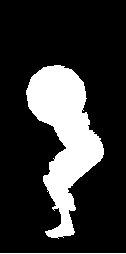
\includegraphics[height= 7cm]{algorithm/images/modelmatchbg}
    }
    \subfigure[Model]{
            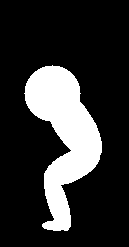
\includegraphics[height= 7cm]{algorithm/images/modelmatch}
    }
\caption{The model (b) is fitted to the background subtracted frame (a)}
\label{fig:modelfit}
\end{figure}

The optimiser does this using an optimisation algorithm and a cost function.

The optimisation algorithm used is BOBYQA, which stands for Bound Optimisation BY Quadratic Approximation. This is an iterative algorithm for finding the minimum value of a function, given a set of bounded variables. The algorithm was developed by M. Powell, and is detailed in his paper\cite{bobyqa}. The algorithm uses the Java implementation of BOBYQA from the Apache Commons Math library\cite{apachemath}.

The main advantages over other multivariate optimisation algorithms are firstly that it does not require derivatives of the cost function, and secondly that it constrains the search space using bounds. With no requirement for derivatives, the cost function can be treated as a `black box', allowing for far more freedom in its design. In the case of this project, the cost function needs to perform operations on the model and video frames, and so it does not have a clear derivative as would a straightforward mathematical function of the input variables. The bounds reduce the search space which speeds up the time taken to find the parameters that best fit the model to the frame. With the right bounds, the chance of the model fitting to the frame in a position that is humanly impossible is reduced.

Another optimisation algorithm that could have been used is the widely known Nelder-Mead method\cite{neldermead}. Whilst Nelder-Mead is also a derivative-free optimisation method, it does not have the advantage of bounds. Bounds could be introduced in the cost function itself, but this would lead to a less predictable cost function, and therefore a more difficult function to minimise. Nelder-Mead is also a slower optimisation method, and performance is a critical factor in this application due to the goal of real-time tracking and analysis. The Apache Commons Math library\cite{apachemath} provides a Nelder-Mead optimisation method, which was trialled for this project but deemed too CPU intensive for real-time processing.

For this application, the speed of the fitting also affects the quality of the fitting. The overall fit across multiple frames is affected both by the quality of the fit to each individual frame, and the number of frames onto which the model is fitted. As the speed of the optimisation in an individual frame increases, the number of frames we are able to fit to also increases. Likewise, as the speed of the optimisation in an individual frame decreases, we are able to fit to less frames in a given time period.

The main BOBYQA parameter that directly affects both the quality and speed of fitting to an individual frame is the number of `interpolation points'. The accuracy and performance trade-off is described in the BOBYQA paper\cite{bobyqa}. In the paper, a value of $2n + 1$, where $n$ is the number of cost function variables (ie. the number of degrees of freedom of the model) is stated as most commonly used to give a good balance of performance and accuracy. However in practice in this application it slowed the fit time for each frame, reducing the frame rate and the quality of the overall fit. Trialling different values, it was determined that the optimal value was the minimum permitted number of interpolation points, $n + 2$. This maximised the frame throughput and although the fit was less accurate per frame, the increased number of frames onto which the model could be fitted gave a better overall fit.

During the development of the tracking algorithm, a few different cost functions were evaluated before settling on the final implementation.

The first cost function attempt was one that returned the sum of the squared distance from each joint in the model to the silhouette of the figure in the frame. The idea behind this was that by minimising these distances, the model's `skeleton' would always remain within the figure's silhouette. This function performed quite poorly, with the model roughly gravitating towards the silhouette, but never fitting properly.

The second cost function attempt was one that calculated the number of overlapping pixels when drawing the model directly on top of the silhouette. The number of pixels that overlap are to be maximised, and so the inverse of this is minimised. That is he number of pixels of background that are not included in the overlap is minimised. Overlap, $o$, is maximised by minimising $(w * h) - o$, where $w$ and $h$ are the width and height of the frame respectively. Overlap is calculated by performing a bitwise AND operation on the binary silhouette frame, $f$, with a binary frame on which the model has been drawn, $m$. This gives a binary frame where values are 1 for pixels that overlap, and 0 for pixels that do not. The number of non-zero pixels are counted to give the overlap value $o$. This gives the cost function:

\centerline{$cost = (w * h) - countNonZero(m \& f)$}

The third attempt was to minimise pixels of the model that did not overlap the silhouette, giving a cost function:

\centerline{$cost = countNonZero(m \& ~f)$}

Although both the second and third cost functions gave good results, the second  seemed to provide the best fit. It is probable that this is due to the larger cost value returned by the second function being less likely to change dramatically for small changes in the model angles. For this reason the second cost function was chosen for the algorithm.

Figure~\ref{fig:modeloverlap} shows the model drawn on top of the foreground frame. Pixels coloured white are those that overlap after running BOBYQA using the chosen cost function. Pixels in grey are those of the model and foreground that do not overlap. The chosen cost function can be visualised as maximising the number of white pixels, by minimising the number of grey and black pixels.

\begin{figure}[H]
    \centering
    \subfigure{
            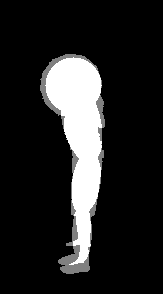
\includegraphics[height= 7cm]{algorithm/images/modelfitstart}
    }
    \subfigure{
            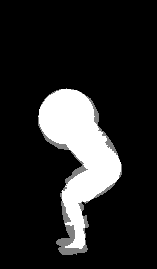
\includegraphics[height= 7cm]{algorithm/images/modelfitmid}
    }
    \subfigure{
            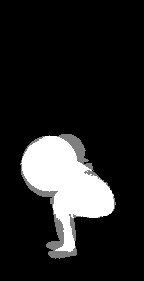
\includegraphics[height= 7cm]{algorithm/images/modelfitend}
    }
\caption{Model fitting by minimising pixels that do not overlap}
\label{fig:modeloverlap}
\end{figure}

At this stage in the algorithm a silhouette and model have been obtained, and through the optimisation the model has been fitted to the silhouette. Therefore on each frame the model is in the same position as the figure performing the squat. This does assume that the fit was perfect, which in practice is not the case, but the fit is generally good enough to assume that the model is in a position reasonably similar to that of the figure.

\subsubsection{Analysis}

The final stage of the algorithm is the analysis. This component of the algorithm examines the angles and positions of the model's joints, to provide information as to whether the model is currently in a good or bad position.

The model provides methods to query its state. An example might be a method that returns whether the hip joint is below the knee joint, allowing us to determine whether the lifter is currently `below parallel' - in the position that they must reach at the bottom of a squat in order for it to be valid. 

On every frame, the model is queried for it's current position, and a global `picture' of the current state of the squat is built up. Exactly how this picture is built up is detailed in section~\ref{sec:listeners}.

The analysis tracks joint positions over time to enable one squat repetition to be differentiated from another. A particular challenge was in how to determine when the lifter is ascending or descending. A simple solution would be to check whether the lifter has just locked out (stood up straight) or has gone below parallel. However in practice a lifter may not perform a correct squat, and may neither squat below parallel nor lock out. The algorithm settled upon was to track the hip joint's vertical motion. As the lifter descends, the hip joint will descend, and as the lifter ascends, so will the hip joint. A fixed size queue of hip joint locations is stored, and on every frame the location is added to the queue (pushing off the oldest hip joint location). This gives a short `history' of hip locations, and we can examine this history to see whether the lifter is currently ascending or descending by checking whether the history is in ascending or descending order. This provides a way to tell when the lifter is ascending and descending, and after each descension and ascension we know that a new repetition has begun.

In the analysis stage, we give each repetition a percentage score, which is calculated by penalising failure to enter required positions (for example going deep enough and standing up straight enough), and also penalising time spent in a sub-optimal or unsafe position (such as leaning too far forward). The time spent is measured in frames, and percentage points are removed from the score based on the proportion of frames in which the lifter is an incorrect position. Each type of incorrect position is given a maximum penalty at which no more percentage points are removed. The maximum penalties chosen are based on the severity of the incorrect position.

As we score each squat, we keep track of the most significant contributor to the score penalty. For example, if 10\% of the score was lost for leaning too far backward, and a 30\% penalty was applied for the lifter's failure to squat low enough, the main contributor would be the fact that the lifter failed to squat low enough. These contributors are stored with each score, enabling the contributor to be shown to the user to allow them to see what the main problem was with their squat. These contributors are used after each rep to provide verbal feedback on how to improve their technique.
\subsection{Termination}
\pagebreak
\section{Implementation}

In this section I will highlight some of the more interesting implementation details and design choices which have contributed to the development, performance and longevity of the codebase.

\section{Development Strategy}

To reduce the learning curve and improve the development process, the core algorithm was first developed for a Linux machine, rather than implementing it as an Android application from the beginning. This allowed a proof of concept to be created early on in the development stages. Video files were read and processed rather than live images from the camera, which gave a more controlled atmosphere for testing. Having never developed an Android application or used OpenCV, developing on Linux first allowed familiarisation with OpenCV development without concern for any Android-specific functionality. With the Linux code all written in Java, the overhead for porting it to Android was minimal.

Platform-specific functionality was abstracted using interfaces during the Linux development process. Once the core algorithm had been completed, the migration from Linux to Android was reasonably straightforward. The Linux implementation of the \texttt{VideoInput} interface (which read frames from a video file) needed to be replaced with an Android implementation (reading frames from the camera). The same needed to be done for the \texttt{VideoDisplay} interface. The OpenCV library for Linux was swapped for its equivalent on Android. Once these steps were taken, the core algorithm ran just as it had done on Linux, which enabled the focus to shift from the algorithm to code optimisation and user interaction.
\section{Events and Listeners}
\label{sec:listeners}

\subsection{Analysis and Scoring}

The observer design pattern is utilised throughout the codebase, but its most interesting use is in the analysis stage.

Upon each iteration of the tracking algorithm, the model's joint positions and angles are examined. This per-frame examination is performed by the \texttt{ModelEventManager}. Other classes may register listener functions with the \texttt{ModelEventManager}, detailing which event it wishes to subscribe to. When a new observation is made on the model (for example we have newly observed that the lifter has gone `below parallel'), an event is triggered, calling every registered listener for that particular event.

The \texttt{ModelEventManager} tracks the state of the model at a low level, providing a high level view to other classes so that they can be notified when the lifter is in a particular position.

There are many events that can be subscribed to, and some of the most interesting ones are listed below:

\begin{itemize}
	\item \texttt{SQUAT\_DESCEND\_START} Triggered as soon as the lifter is detected to be descending.
	\item \texttt{SQUAT\_ASCEND\_START} Triggered as soon as the lifter is detected to be ascending.
	\item \texttt{SQUAT\_BELOW\_PARALLEL\_START} Triggered as soon as the lifter goes low enough.
	\item \texttt{SQUAT\_BELOW\_PARALLEL\_END} Triggered as soon as the lifter travels upwards out of the below parallel state.
\end{itemize}

There are many other events (listed in the appendix in section~\ref{sec:appendix_events}) that are triggered when the lifter first enters and exits a position of bad form.

This design pattern allows a high level way to track the lifter's position. For example one could write a simple class to count the number of repetitions a lifter performs, with no need to worry about checking each frame. This example might look as follows:

\begin{lstlisting}[style=javastyle]

public class SimpleRepCounter {
	private int reps = 0;

	public SimpleRepCounter(ModelEventManager manager) {
		manager.addListener(ModelEventType.SQUAT_DESCEND_START,
			new ModelEventListener() {
				public void onEvent(Model m) {
					reps++;
				}
			});
	}

	public int getReps() {
		return reps;
	}
}

\end{lstlisting}


The more advanced components used in the analysis and scoring of each repetition use sets of listeners in a similar manner.

The \texttt{ModelEventManager} provides a simple way to add new analysis functionality, whether at the low or high level.

\subsection{Other Listeners}

The remainder of the codebase uses listeners in order to update the user interface or provide the user with real-time feedback. This pattern was used to ensure that the core algorithm was separated from the user interface. The user interface registers itself as a listener to the \texttt{SquatPipeline}, which calls different listener functions at different stages of the algorithm. Example uses include updating the notification text in the user interface or emitting a beep whenever the lifter squats low enough.
\section{Optimisation}

In order to track and analyse squats in real-time, the code needed to be optimised. This was particularly important after the port to Android, where the limited hardware of a mobile device made inefficiencies more apparent.

\subsection{Memory Management}

The OpenCV website provides a short set of guidelines for best practices in using their libraries on Android\cite{opencvoptim}. The main practices encouraged are to avoid repetitive Java Native Interface (JNI) calls into C++ code, and to avoid excessive memory allocations by initialising matrices towards the start of the application, reusing them rather than reallocating them upon every use.

Matrices in OpenCV are defined as \texttt{Mat} objects. In order to follow the best practices for allocating and using \texttt{Mat} objects, a class called \texttt{MatManager} was created. The \texttt{MatManager} is a static class though which the codebase retrieves matrices. It has a single function, \texttt{get()} which returns a reference to a \texttt{Mat}. This \texttt{get()} function takes a string key as a parameter, and keeps track of a map of these keys to \texttt{Mat} objects. When requested for a matrix with a key that does not exist in the map, the matrix is created, and when the key does exist, the matrix that has previously been created is returned.

The \texttt{MatManager} made it very simple to modify the code to reuse matrices. Wherever the codebase had previously created a \texttt{Mat}, the construction was replaced with \texttt{MatManager.get()} and an appropriate key.

The use of \texttt{MatManager} dramatically increased the speed of the application on Android, allowing tracking and analysis to occur in real-time. It avoids the allocation of more memory than the application needs, and the overhead of garbage collection to clear the memory space of dereferenced matrices. Each allocation of a matrix also requires a JNI call, and so these were also minimised.

\subsection{Model Fitting}

A small but powerful factor in improving the performance of the application was the maximum number of iterations that the BOBYQA optimiser was permitted to perform. When unbounded around fifty iterations were completed before the best fit was found for every frame. Some frames required a far higher number of iterations, in some cases an order of magnitude larger than the norm. This would cause the application to freeze temporarily, as this CPU intensive process was performed for many iterations. To avoid this it was required to cap the number of iterations to a sensible value.

Capping the number of iterations at too high a value would mean that in the worst case the frame rate would be slow, giving the user a poor experience. Too low a value would mean that the fit per frame would not be accurate enough, causing the model to poorly follow the figure and give bad analysis results.

A good value which met this trade-off was twenty iterations. This gave a precise  enough fit and a fast frame rate. The faster frame rate also meant that the fitting could run on more frames, giving a better overall fit over time.

\subsection{Point Cache}

In order to draw the model, the start and end points of each ellipse must be calculated based on the coordinates of the toe and the angle of each joint. This is performed using simple trigonometry, taking the angle and length of each component to generate each point.

These points are queried several times per model state in order to check the form of the squat. To avoid recalculating the points upon every query, the points are stored in an array when first calculated. Every time thereafter the points are retrieved directly from this array, until the model's angles are adjusted by the optimiser and the array is cleared.

This provided a reasonable speed-up due to the high frequency of calls to the point calculation function.
\pagebreak
\section{The Application}

In this section I will detail how a user might go about using the application and explain some of the features from a user perspective.

\subsection{User Workflow}

The steps that a user of the application will follow are detailed in this section.

\begin{figure}[H]
    \centering
	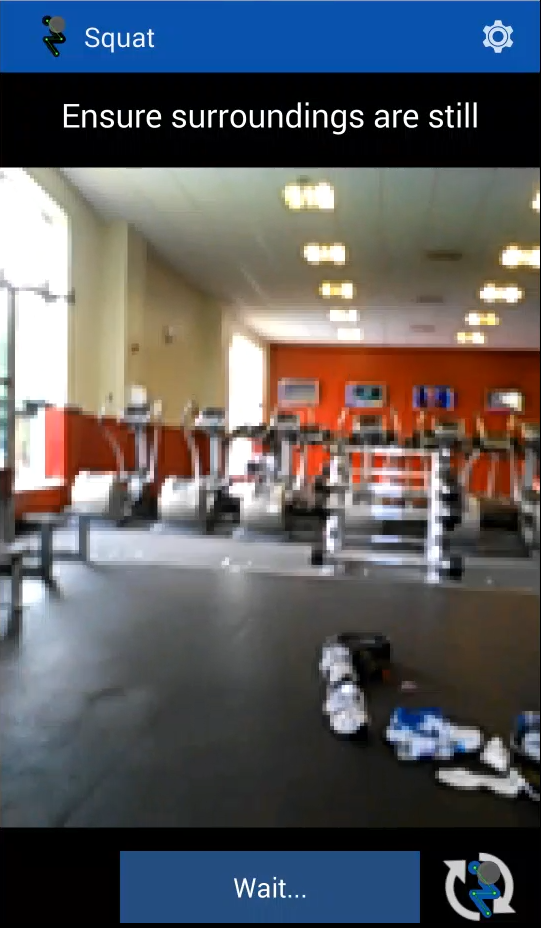
\includegraphics[height=10cm]{application/images/ensuresurroundingsstill}
\caption{Wait until the device and its surroundings are still}
\label{fig:ensuresurroundings}
\end{figure}

The user begins by starting up the application. They will immediately see a video feed of the front-facing camera of their Android mobile device. They will see a message at the very top of the screen, instructing them in the first step they must take: ``Ensure surroundings are still''.

A button at the bottom of the screen displays the text ``Wait...'', indicating that some action must be performed before the button can be pressed. Figure~\ref{fig:ensuresurroundings} shows this screen.

\begin{figure}[H]
    \centering
	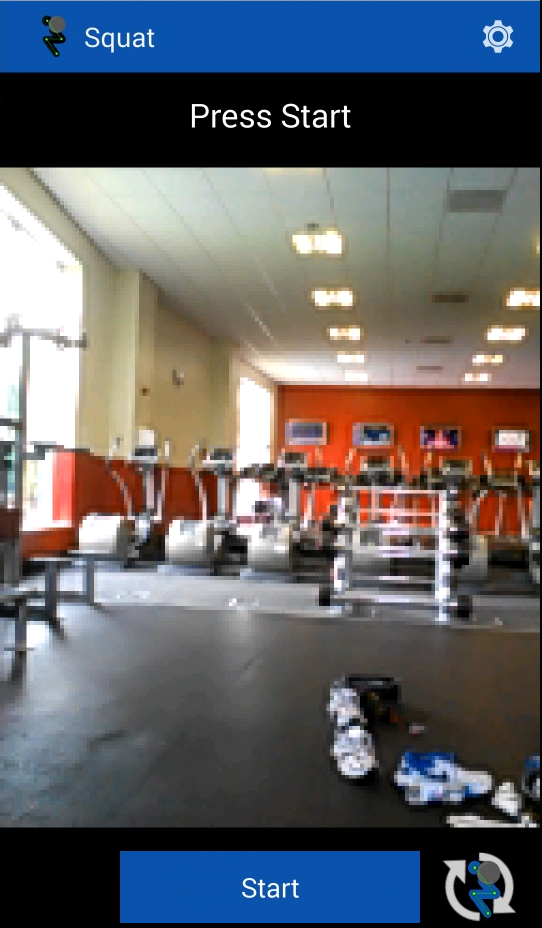
\includegraphics[height=10cm]{application/images/pressstart}
\caption{The background is deemed still, allow the user to press start}
\label{fig:pressstart}
\end{figure}

As the user follows the on-screen instruction of ensuring that their surroundings are still, they will notice that the instruction text changes to ``Press Start'' automatically, and the button displays ``Start'' and is lightened to indicate that it may be pressed. This screen is shown in figure~\ref{fig:pressstart}.

This initial stage of disabling and enabling the button ensures that the user places their phone in a location where it will not move, to allow background subtraction to work effectively. It also ensures that there is no movement in the background, which may distort the background subtraction and cause the model to `lock on' to a different figure.

The application tolerates a little movement, meaning that movement too far away to cause background subtraction issues is allowed. This avoids the frustration of a user requiring an area completely devoid of movement to use the application.

\begin{figure}[H]
    \centering
	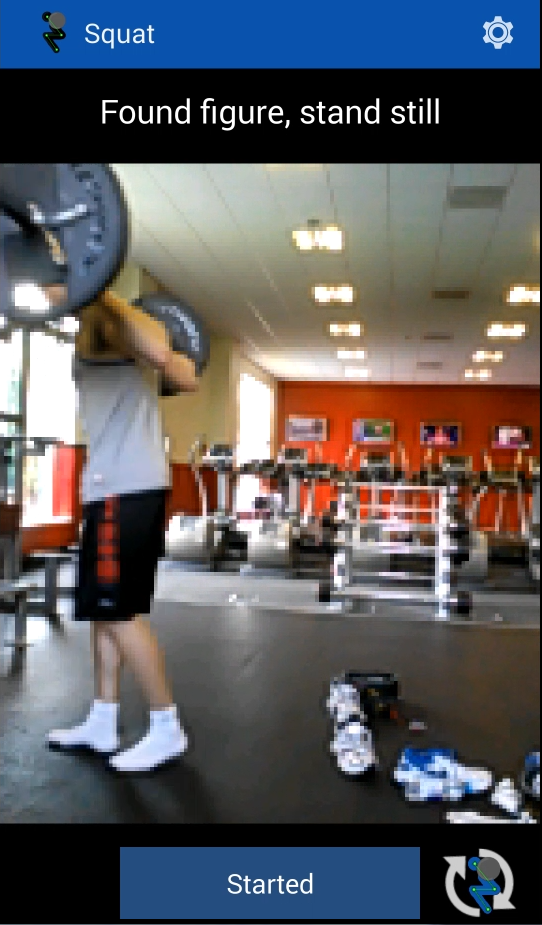
\includegraphics[height=10cm]{application/images/foundfigure}
\caption{A figure has been detected}
\label{fig:foundfigure}
\end{figure}

As a side note, there is also a button to the right of the start button. This button is used to flip the expected orientation of the lifter. It defaults to expect the lifter to face left (as they look at the screen). When this button is pressed, the figure in the icon flips to indicate that the lifter must stand facing the opposite direction. Vocal feedback is also used, with a voice saying ``Face left.'' or ``Face right.'' to confirm this change of orientation.

Once the start button is enabled, the user presses the button, and immediately receives vocal directions to ``Walk into view and stand still, facing left'', as well as the instruction text changing to ``Walk into view''. The vocal instruction here will say ``Walk into view and stand still, facing right'' should the orientation have been changed by the user.

The user will follow these instructions, collecting their barbell from the squat rack out of view, and walking into the application's view. As the user walks into view, the instruction text will update to indicate that the user has been recognised by the application: ``Found figure, stand still''. This is shown in figure~\ref{fig:foundfigure}.

\begin{figure}[H]
    \centering
	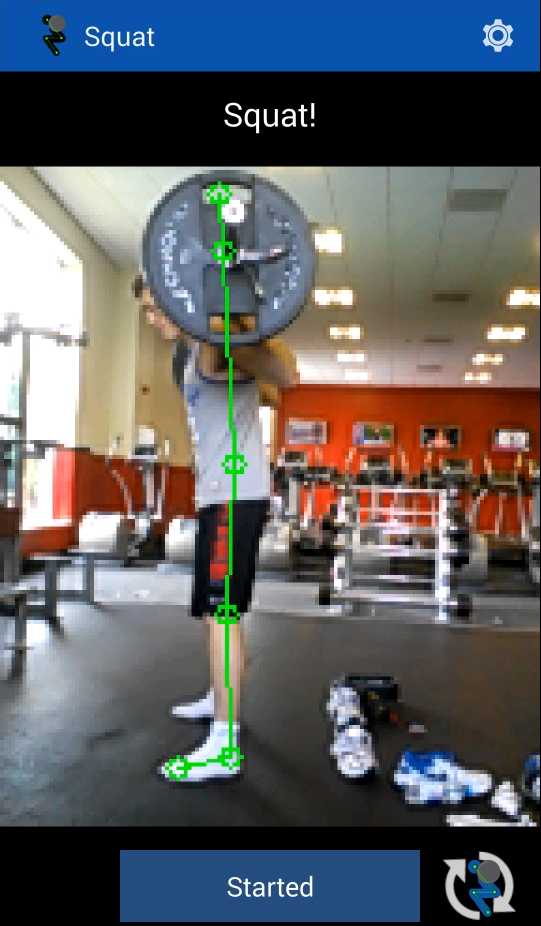
\includegraphics[height=10cm]{application/images/startsquatting}
\caption{The model is mapped to the figure once the figure is still}
\label{fig:startsquatting}
\end{figure}

Once the user has moved into position, and stood still following the instructions, the application will emit a beep as it fits the initial model to the user. As it does this, the video feed will add an overlay showing the model drawn as a skeleton - with lines connecting points in a stick figure fashion. Although this is not the model drawing method used in fitting, it is more intuitive for the user to see a skeleton view than the model constructed of ovals. This encapsulates the underlying functionality, displaying the model in a user-friendly way. From this, the user can see that they have been recognised by the application, and that the application has started to track their movement. Figure~\ref{fig:startsquatting} shows this stage.

\begin{figure}[H]
    \centering
	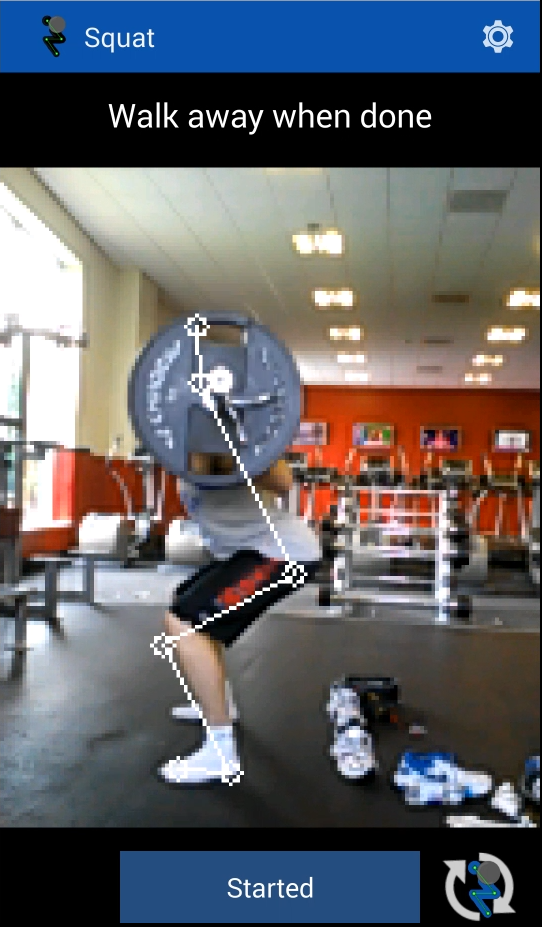
\includegraphics[height=10cm]{application/images/midsquat}
\caption{The skeleton tracks the lifter's movement throughout the squatting phase}
\label{fig:midsquat}
\end{figure}

As the model is displayed and the application beeps, the application's voice will indicate the next move expected from the user by saying ``Start squatting when ready.''. The user may now begin squatting in their own time. As they squat, the skeleton on screen will be updated in real-time as the tracking part of the algorithm runs, as shown in figure~\ref{fig:midsquat}.

\begin{figure}[H]
    \centering
	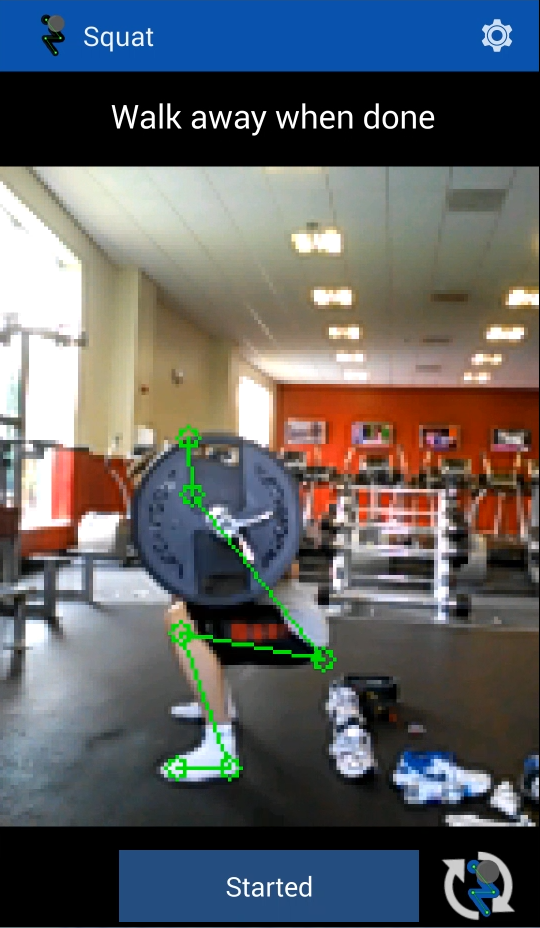
\includegraphics[height=10cm]{application/images/belowparallel}
\caption{The skeleton is drawn in green to indicate that the squat is low enough}
\label{fig:belowparallel}
\end{figure}

As the user descends low enough for the squat to be considered valid, the application emits another beep. This real-time feedback is incredibly useful, meaning that the user will know when they have squatted low enough during the movement, rather than only discovering this after they have finished their set. When hearing a beep, the user knows immediately that they must start the ascension part of the movement and can begin to drive with their legs. On-screen, the skeleton changes colour to green (as shown in figure~\ref{fig:belowparallel}), reinforcing the notion that their squat is low enough to be considered valid.

\begin{figure}[H]
    \centering
	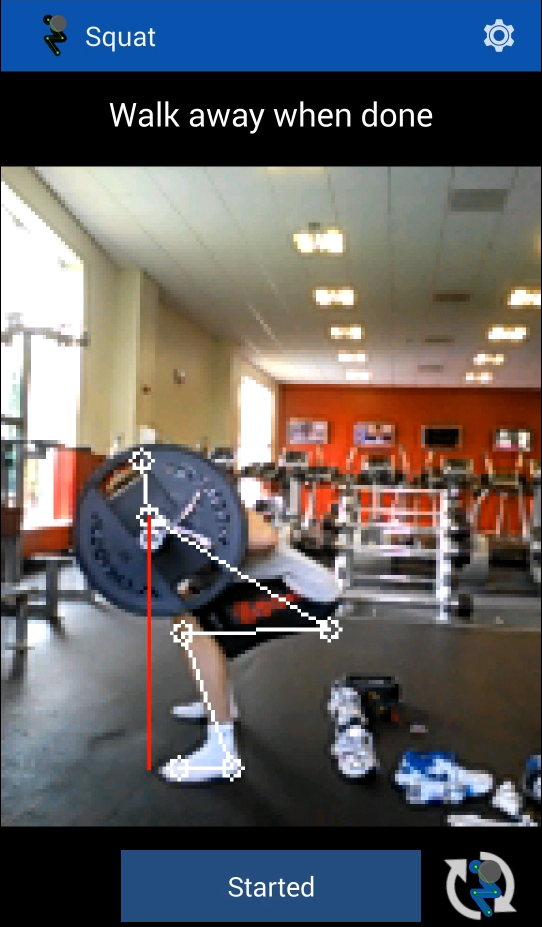
\includegraphics[height=10cm]{application/images/weightdistro}
\caption{A red line indicates sub-optimal weight distribution}
\label{fig:weightdistro}
\end{figure}

Another element of visual feedback is a line which shows the weight distribution of the squat. For a squat to be optimal, the bar must be directly above the feet at all times, giving the user maximum leverage to support the weight. Should the application detect that this is not the case, and the weight is too far in front of the lifter's toes, or too far behind the lifter's heels, a red vertical line is drawn from the bar to the feet, as shown in figure~\ref{fig:weightdistro}. This traces the weight's position above the feet, showing that it is too far forward or backward.

\begin{figure}[H]
    \centering
	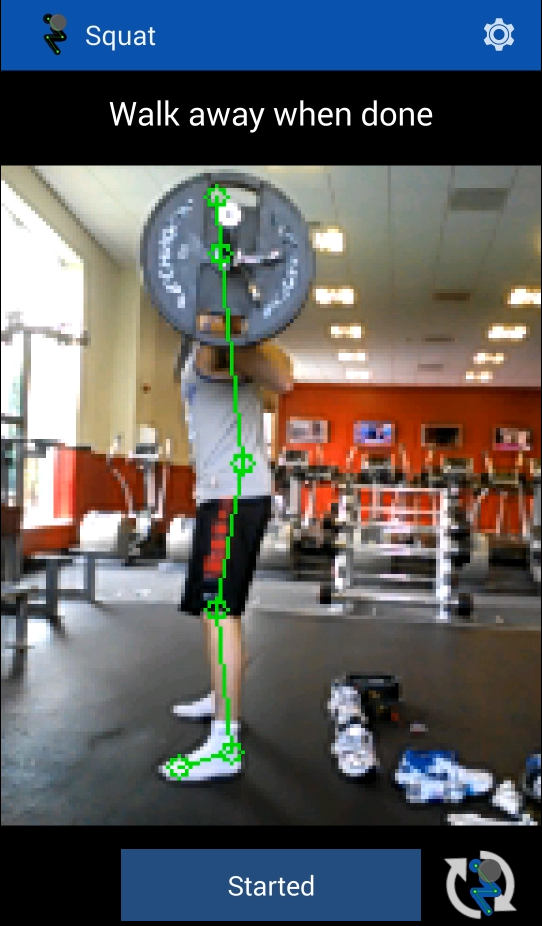
\includegraphics[height=10cm]{application/images/lockout}
\caption{The skeleton is drawn in green and vocal feedback is given as the lifter locks out}
\label{fig:lockout}
\end{figure}

As the user completes the ascension part of the squat (thus completing one full repetition) and `locks out', the skeleton is again coloured green as shown in figure~\ref{fig:lockout}. At this point, the application detects that a repetition has been completed, and provides the user with vocal feedback. This vocal feedback includes the current rep number, how successful the squat was, and a tip on how to improve the squat if necessary. An example might be ``Two. Good. Try leaning forward a little more.'', or ``Four. Ok. Try squatting deeper.''.

So as not to bore the user with the same repetitive messages, slight variations of each tip are chosen at random, depending on the main problem with the squat. For example if the user fails to squat deep enough, they may be told to ``Squat deeper.'' or ``Try to squat below parallel'' or one of many other variations.

The part of the feedback which tells the user how well their squat was performed overall can be one of the following: ``Not very good.'', ``Ok.'', ``Good.'', ``Very good.'', ``Excellent'', ``Perfect''. These are selected based on the score for the rep that they have just completed. For example, ``Very good.'' is said should the user achieve a score between 70\% and 90\%. When a user achieves a score above 90\%, the verbal feedback will not provide the user with a tip. This gives the user a more satisfying experience, encouraging the user to strive towards good squatting technique.

\begin{figure}[H]
    \centering
	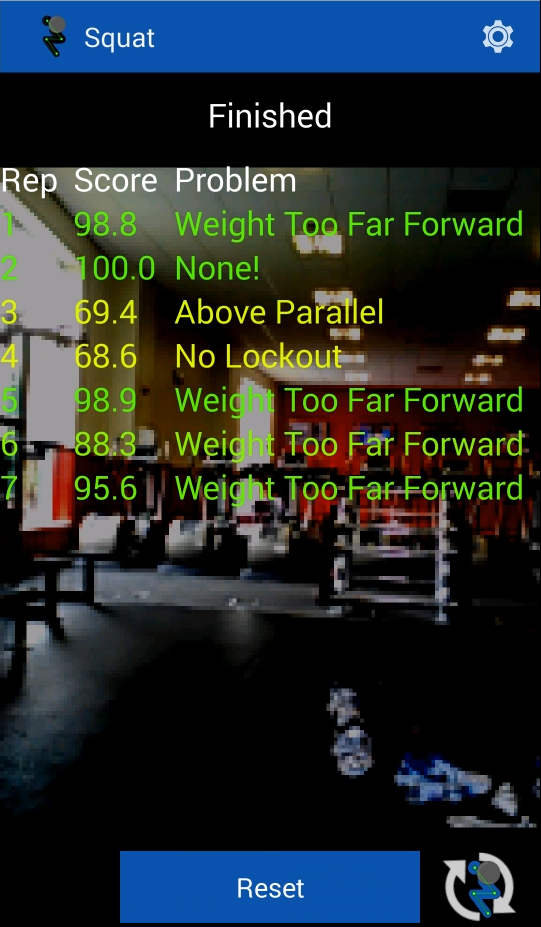
\includegraphics[height=10cm]{application/images/scores}
\caption{The lifter's scores are displayed once they have finished squatting}
\label{fig:scores}
\end{figure}

This process repeats for every repetition completed by the user. Feedback is given as the figure is detected to stand up straight or, should they fail to fully lock out, as they begin descending into their next repetition.

When the user has completed their desired number of squats, they simply walk out of view. This follows the usual procedure, where a lifter will place the weight back in the rack on the completion of their set of squats. As they walk away, the tracking and analysis phase will end, and a breakdown of their scores is displayed on the screen as shown in figure~\ref{fig:scores}.



Here, the user can see their score for each repetition they completed, and also the main `problem' with their squat. Each entry in the table is coloured in relation to its score, giving the user an instant visual indication as to how well their squat was performed, without the need to read each score value. A set of scores that is mostly green will indicate to the user that they performed a good set of squats, and a largely orange or red set of scores will inform the user that they should improve their technique.

Once the user has reviewed their scores, they can press the reset button. This will change the application to its initial state, allowing the user to press the start button once their surroundings are still.
\subsection{Customisation}

Users are given several options in the settings to customise their experience. The majority of these settings are given to allow the user to customise the real-time feedback they receive. They can choose any combination of repetition counting, vocal feedback and tips, vocal instructions to direct them, and beeps to indicate detection and that they have descended low enough. Figure~\ref{fig:settings} shows some of the feedback options available to the user.

\begin{figure}[H]
    \centering
	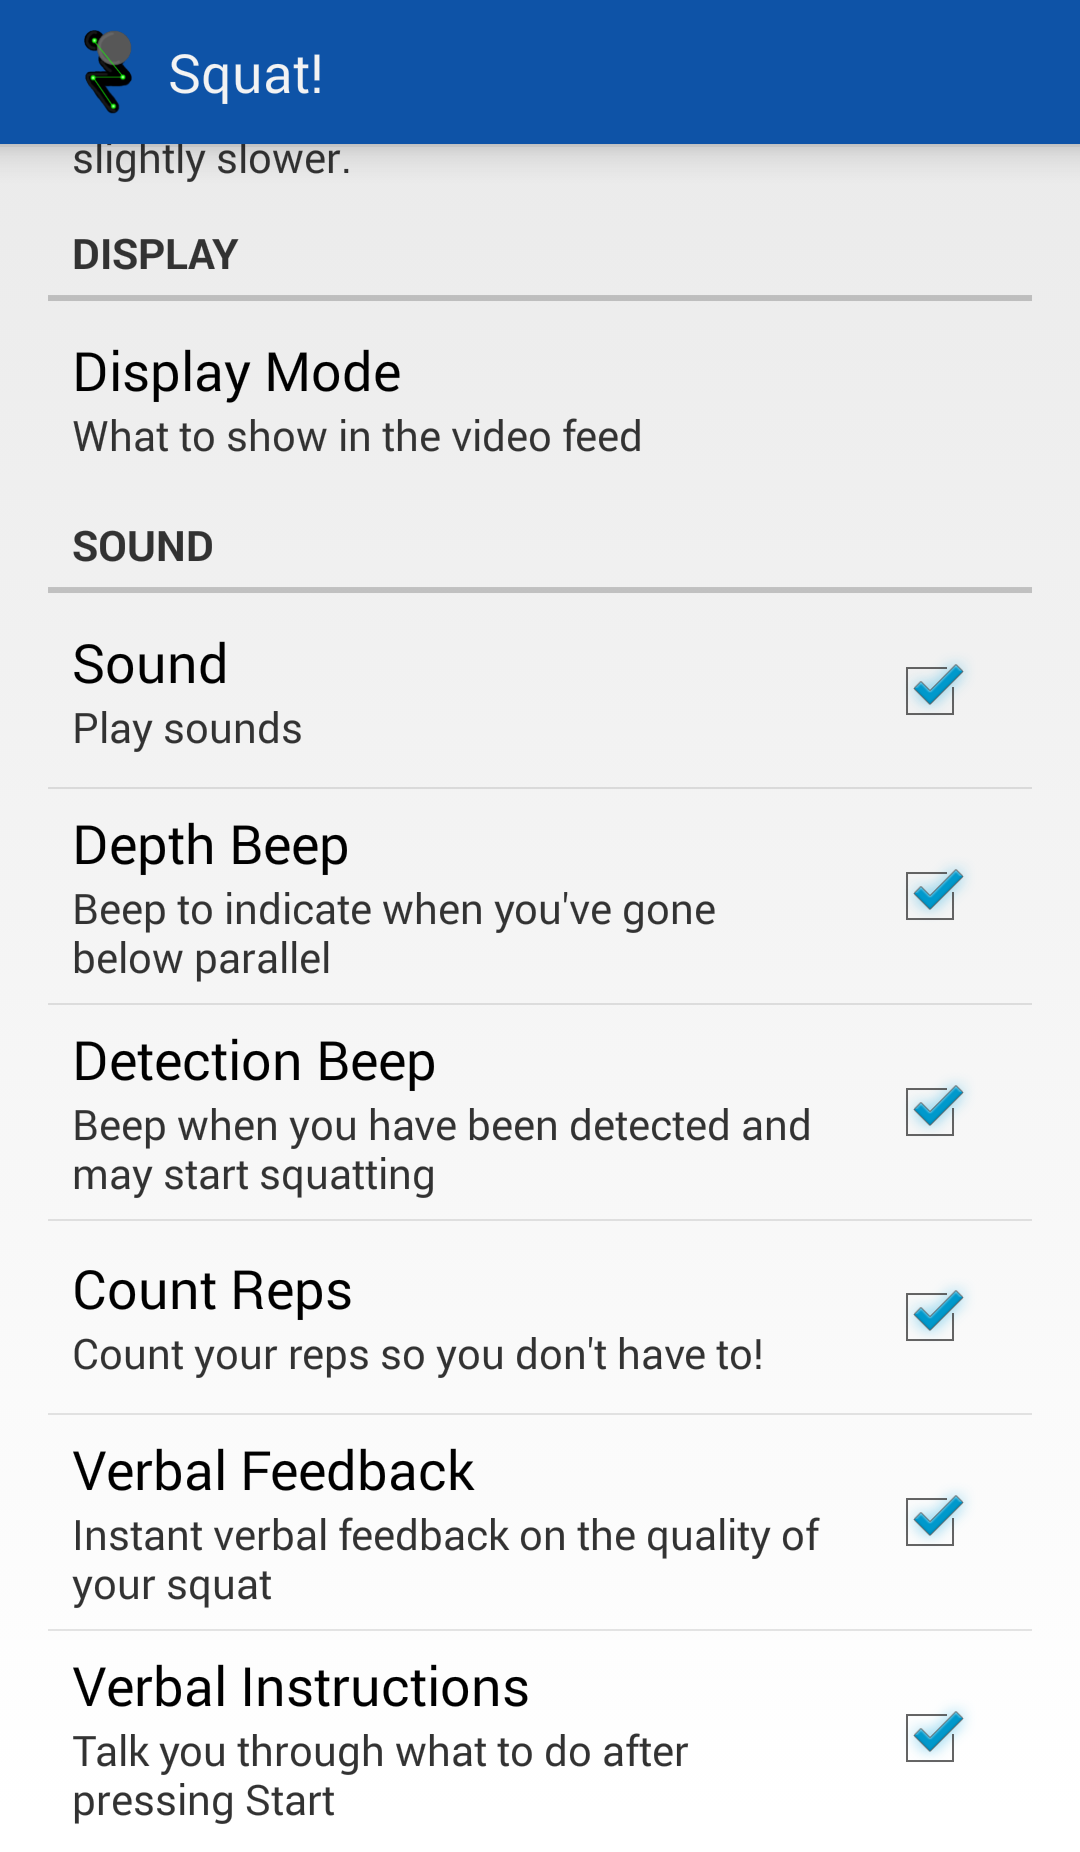
\includegraphics[height=10cm]{application/images/settings}
\caption{Some of the settings available to the user}
\label{fig:settings}
\end{figure}

The user is also given the ability to customise the detection stage of the algorithm, setting the detection's motion sensitivity and detection time. The motion sensitivity dictates how still the lifter must be in order to be detected and for the initial model fit. The detection time dictates how long the lifter must stand still before the model is mapped to them and they can begin squatting. This customisation allows the user to choose whether they prefer to walk out and start squatting quickly, or whether they might take a little longer to get into position and adjust their foot placement.

The user is also given a `Squatting With Barbell' checkbox. This allows the user to select whether or not they are squatting with a weight on their back, and the model will draw the weight on its shoulders if selected. This allows the user to practice squatting without a barbell, and gives better tracking results for that case.

Settings are implemented using Android's Preferences API, which ensures that changes made to the settings persist.
\pagebreak
\section{Evaluation}

\subsection{Goals}

My goals for this project are to have an easy to use application that will give real-time feedback on the execution of a squat and deadlift. The application should be non-intrusive, requiring no special equipment. It should be reasonably accurate, able to notify the lifter when they have executed a lift correctly or not.

\subsubsection{Squat Feedback}

The following feedback should be given to inform the user whether or not their squat was valid:

\begin{itemize}
	\item \textbf{Depth} Whether or not the hip joint goes below the knee at the bottom of the squat
	\item \textbf{Lockout} Whether or not the lifter fully locked out their knees and hips to finish in an upright position
	\item \textbf{Reverse Movement} Whether or not the lifter moved downwards in the ascent part of the squat
\end{itemize}

The following feedback should be given to inform the user whether or not their squat was safe:

\begin{itemize}
	\item \textbf{Upright Shins} Whether the shins remain near-vertical throughout the lift (to avoid knee injury)
	\item \textbf{Back Flexion} Whether the spine remained neutral during the lift (to avoid back injury)
	\item \textbf{Back Angle} Whether the back remains within an optimal range of angles during the lift
\end{itemize}

\subsubsection{Deadlift Feedback}

The following feedback should be given to inform the user whether or not their deadlift was valid:

\begin{itemize}
	\item \textbf{Lockout} Whether or not the lifter fully locked out their knees and hips to finish in an upright position
	\item \textbf{Reverse Movement} Whether or not the lifter moved downwards in the ascent part of the deadlift
\end{itemize}

The following feedback should be given to inform the user whether or not their deadlift was safe:

\begin{itemize}
	\item \textbf{Back Flexion} Whether the spine remained neutral during the lift (to avoid back injury)
\end{itemize}

\subsection{Testing}

To test the core functionality of the app, I will provide a sample of gym-goers with a copy, and ask them to review it according to the following criteria:

\begin{itemize}
	\item Ease of Use
	\item Accuracy
	\item Effectiveness (ie. how much it helped their training)
\end{itemize}

To evaluate whether the application runs in real-time, I will benchmark test the frames per second of the application. A value above 10fps will be considered a suitable frame rate.

I will also test its accuracy by running the application against good and bad squats, and recording the number of true positives, false positives, true negatives and false negatives. These results will be used to give statistics on the success of the project.
\pagebreak
\section{Conclusion}
\pagebreak
\section{Future Work}
\label{sec:future}

\subsection{Improvements to the Application}
\label{sec:improvements}

In light of the evaluation, there are several improvements that could be made to the application.

\subsubsection{Background Subtraction Algorithm}

One of the points raised in the evaluation was that the model would sometimes stray from the figure whilst tracking. This seemed to be due to fluctuations in the lighting of the room. Most gyms have even lighting, but the ambient lighting would gradually change over time (for example the sun outside emerging from clouds) causing the background pixels to change their colour.

This issue could be addressed by using a more adaptive background subtraction algorithm. One proposal for this algorithm is to take the pixels that have been determined not to be foreground and updating these pixels in the background model to a weighted average of the previous value and the new value. This would give us a background model which changes over time, allowing for gradual changes in lighting.

Another point raised in the evaluation was the difficulty in using the application in a busy gym during peak times. The application is robust to a certain degree of movement in the background during the tracking and analysis phase, meaning that a figure walking into view or performing an exercise in the background will not affect it too much. However when the application first loads, it must be placed in a still location, and in order to check that the application is still, it uses the camera to make sure that there is no motion in the feed. This means that the application must point to a clear area in order to start.

An option to avoid this requirement in the detection phase might be to switch off the motion detection and allow the user to start the processing at any time. This would not be as intuitive, as the user will not be as well informed that the phone must be placed in a still location.

Another option might be to use the Android API to access the accelerometer of the mobile device, checking its readings to detect when the device is set up correctly.

\subsubsection{Tracking}

Although the tracking was reasonably robust, the model did not always fit to the lifter throughout the entirety of the repetition, causing the 17 poorly tracked squats out of the 84 used in the evaluation (section~\ref{sec:analysis_eval}). A future improvement might be to investigate ways to improve the tracking. The problems are likely due to changes in lighting conditions, but there may be other factors which affect tracking.

An improvement might be to have the algorithm detect when a repetition was tracked incorrectly, offering no feedback for the squat.

\subsubsection{Squat Rack}

Many lifters will perform their squats within the squat rack, which provides bars to catch the weight should they fail to execute the lift. These bars obstruct the view of the lifter, and therefore the current tracking algorithm cannot follow a lifter inside the rack. Figure~\ref{fig:squatrack} shows the application failing to track the lifter inside a squat rack.

\begin{figure}[H]
    \centering
    \subfigure{
            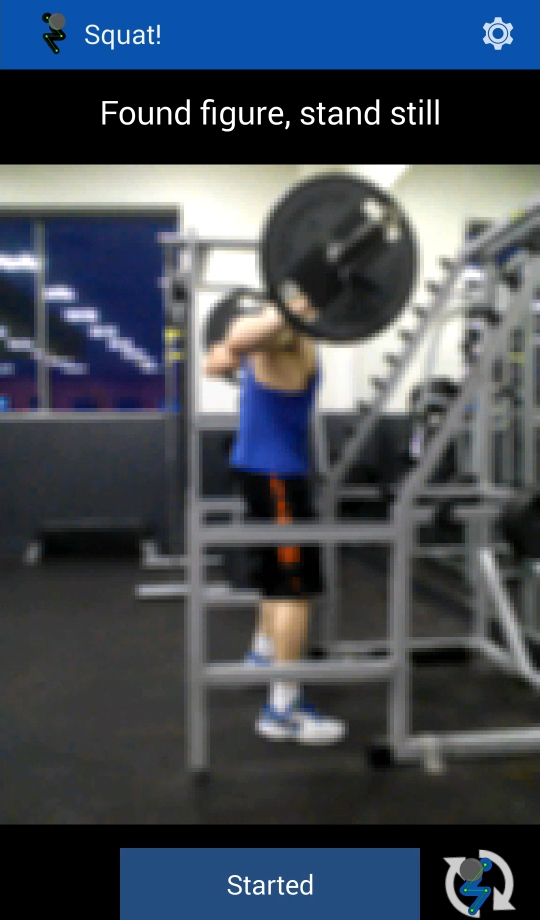
\includegraphics[height= 9cm]{future/images/squatrack}
    }
    \subfigure{
            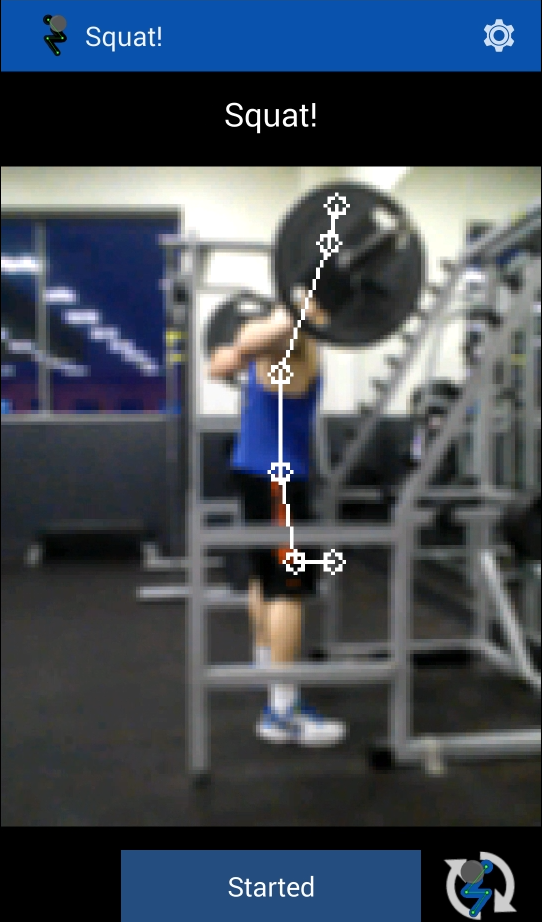
\includegraphics[height= 9cm]{future/images/squatrackfail}
    }
\caption{Tracking fails with stationary obstructions such as a squat rack}
\label{fig:squatrack}
\end{figure}

This is not a major problem, as many lifters will be happy to perform their squats away from the rack, especially during times of training when lifting a weight that they know they can squat easily, without the worry of failing. When a lifter attempts a new personal record or a weight they are unsure that they are able to lift, they will use the squat rack. In this case they would not be able to use the application.

A future enhancement to the application would be to adjust the algorithm to allow for stationary objects in front of the lifter. One option which might allow for this may be to `join' objects detected as foreground that are reasonably close to one another, so as to create a full figure from the parts of the figure that can be seen.

\subsubsection{Resolution}

At present the resolution of the application is fairly low. Higher resolutions were tested, but the increased number of pixels reduced the reliability of background subtraction, often causing the figure to be segmented and poorly tracked.

The primary disadvantage of a low resolution is the low quality of the frames displayed to the user. In order to maintain the performance of background subtraction and the speed increase of processing fewer pixels, a future extension might be to display higher quality frames than are actually being processed. The algorithm could run on low quality frames, whilst displaying the model scaled to fit to the larger frame. This would have a minimal impact on the speed of the application, no impact on the tracking and provide the user with higher quality frames to give the application a more professional feel.

\subsubsection{Model Proportions}

The model is scaled to fit the lifter using a single scale factor, determined during the detection phase of the algorithm. Whilst this single scale factor adjusts the size of the model to fit the lifter, it does not adjust the model's proportions.

Through user testing, it was found that tracking is fairly robust for users with different proportions. However tracking could be improved by adjusting the models proportions to fit the lifter. It is a difficult challenge in computer vision to find the lifter's joints in order to automatically set the model's proportions, but this is something that could be investigated further to provide a more intuitive experience.

Another option might be to allow a user to set the model's proportions in the settings. This could be a simple process of inputting measurements (which would require a tape-measure) or perhaps a more interesting way would be to prompt the user to take a photo of themselves side-on using their mobile device, and have them mark their joints by tapping each joint location. The model could be drawn onto the screen as they tap, and the user could drag the joints to fine tune them once finished.

As well as proportions length-wise, the model's stature could also be adjusted in the settings. This may provide better tracking and analysis for lifters of varying weight.

\subsubsection{Model Degrees of Freedom}

Another future enhancement to the application might be the introduction of a more advanced model. The model currently has five degrees of freedom that the optimiser will use to adjust the model to fit the figure. This works well in practice, and gives enough information to analyse the majority of factors affecting squat form.

The spine is currently modelled as a rigid line from the shoulder/neck area to the hip. Of course this is not the case in the human body, where the spine is made up of a series of vertebrae. The spine can bend in an arc both forwards and backwards, and this can occur during squats. Perhaps a model which treated the spine as a series of connected vertebrae might track the figure better. This would also provide the ability to check whether the lifter's back was rounded in a squat, which can cause injury.

An increase in the degrees of freedom will have a detrimental effect on the performance of the fitting, giving it more variables to optimise over.

\subsubsection{Recording for Further Analysis}

An interesting idea for a feature mentioned by users in section~\ref{sec:user_testing} was the notion of recording the output of the application for later viewing. This would then allow the user to review their squat form themselves and check whether the model tracked them accurately enough to see if its feedback is genuine.

The ability to replay a squat with an overlay of a skeleton would be a very helpful way for a lifter to review their form and learn how to improve their squats. Should this be done, it may also be worth implementing more visual feedback displayed on the screen. Joints and angles of interest could be highlighted, and labels could show the particular issues with form during the lift. At present, the application shows a `weight distribution line' from the centre of the weight down to the lifter's feet when the weight is in an incorrect position, but this visual form of feedback could be expanded upon in line with the verbal feedback.

\subsubsection{Voice Commands}

A way in which the level of physical interaction with the application could be minimised might be through the use of voice commands. At present once the lifter has placed their device in a still location with a clear view of the lifting area, the lifter must press the `Start' button. They then walk into view, and are detected when they stand still in clear view. Pressing the start button could be eliminated via a `Start' voice command, which would mean that once the lifter has placed their device, they no longer need to physically interact with it until they have finished using it.

Instead of automatically fitting the model to the lifter after standing still and in view, the lifter could initiate the initial fitting with a voice command. This would allow the lifter to spend more time setting up for their lift, which would be particularly useful should they like to make small adjustments to the placement of their feet.

Other voice commands could be used during the squatting phase should the lifter realise they did not set their preferences as desired. For example if after their first repetition the lifter realised they did not have the sound on, they could issue a command to switch it on and continue their set with verbal feedback.

Voice commands may be impractical in the environment of a gym however, as the sound of music and machines may mean that the application cannot hear the lifter. The distance of the lifter to the device may also cause the commands to be distorted.

\subsubsection{Other Lifts}

As well as general enhancements to the current algorithm and application, there are many other lifts that could be introduced, each with their own factors affecting their form.

The deadlift and bench press are the other two powerlifting techniques that would be useful to analyse. Deadlifts would be particularly useful, being an advanced technique that often causes back injury due to incorrect form. A particular challenge with deadlifts might be that the bar is usually placed in the lifting location prior to the lifter entering the scene. This is unlike a squat, where the lifter and bar will enter the view together. With the current algorithm, the bar would be detected as background whilst on the ground, and only as foreground once it left the ground. A very similar model could be used, only requiring the addition of arms to the current model used for squats.

The bench press would come with other challenges. A different viewpoint may be required to check whether the lift has been executed correctly - factors such as the position of the bar along the lifter's body, the angle of the lifter's elbows, whether the bar touched the lifter's chest and many others cannot all be determined from the same viewpoint.

Other lifts that this technology could be applied to are the Olympic weightlifting techniques. The two Olympic weightlifting techniques are the `clean and jerk' and the `snatch'. These lifts are more complicated than the powerlifting techniques, with several stages to each lift with the goal of raising the bar above the lifter's head. Each of these lifts however could be monitored side-on with a monocular camera to check the majority of factors determining the safety and validity of the lift. Whilst powerlifting techniques are used a lot in general training at the gym (whether for sport or recreationally), Olympic weightlifting techniques are more commonplace in a professional environment. This might mean that there is scope for other methods such as the use of a stereo camera or Kinect to separate the lifter from their surroundings and to track the technique in a three-dimensional way. 

\subsubsection{Social Network}

Perhaps another future enhancement to this application would be to build a social network around it. This could allow users to share scores and compete with one another, encouraging them to work on their squat form and to keep training at the gym.

This idea could be taken even further, with the possibility of sharing videos of their tracked squats. This way lifters would be able to receive feedback from a community of gym-goers as well as from the analysis of the application. Human observers would be able to provide a more accurate critique of squat form and will be able to pick up on errors that are too subtle to be detected by the application.

This would enrich the overall user experience of the application and provide users with even better feedback.

\subsection{Launch}

In the not too distant future, the aim is to launch the application to the general public, placing it on the Google Play\cite{googleplay} store. The application is in a good state to release immediately, but some of the improvements mentioned in section~\ref{sec:improvements} may be added prior to launch.

There has been some online interest in the application since a video demonstration of the application was uploaded to YouTube\cite{youtube}. Particular interest was shown on a few threads on Reddit\cite{reddit}\cite{redditpopularity}, which linked to the video. Comments included:

\begin{quote}
\emph{Give me this already!}
\end{quote}

\begin{quote}
\emph{I'd love to see this and one for deadlifts!}
\end{quote}

\begin{quote}
\emph{This is phenomenal, and I wish it were almost required at some gyms. I see some kids doing some nasty Squats that they are gonna regret when they get older.}
\end{quote}

From these comments and many more, it can be seen that this application will be very useful and I look forward to launching it and continuing to develop it in the future.

\subsection{Other Applications}

The technology used in this project has applications outside of weight lifting, in both sports and other areas.

\subsubsection{Sports}

Within sports there is a very wide scope for figure tracking and analysis.

One particular application might be for cyclists training on a rolling road. A particularly important part of the cyclist's technique is to keep their torso close to the bike to minimise drag. Tracking and analysis could be used to determine whether the cyclist is in the correct position, indicating when they rise up into a sub-optimal position in real-time.

There is also scope for use in gymnastics, where weight distributions could be analysed to aid gymnasts in their technique, prompting them to lean more in a particular direction.

\subsubsection{Other Fields}

Other uses for real-time body tracking might be in interaction with user interfaces and games. Kinect already shows the popularity of this kind of technology, but this is lacking in the mobile industry. This technology could be applied to interacting with the interface of a mobile phone via the use of gestures, or perhaps in a game to allow you to adjust the pose of a character by moving your own body.


\pagebreak
\chapter{Appendix}

\section{Verbal Feedback}
\label{sec:appendix_feedback}

Verbal feedback is given according to the score brackets shown in figure~\ref{fig:score_brackets}:

\begin{figure}[H]
    \centering
	\begin{tabular}{ | c | c | }
		\hline
	    \textbf{Score (\%)} & \textbf{Feedback}\\ \hline
	    [0,30) & Not very good \\ \hline
		[30,50) & Ok \\ \hline
		[50,70) & Good \\ \hline
		[70,90) & Very good \\ \hline
		[90,100) & Excellent \\ \hline
		100 & Perfect \\ \hline
	\end{tabular}
\caption{Score brackets for verbal feedback}
\label{fig:score_brackets}
\end{figure}

Tips are given when a problem is detected with a squat and the score is below 90\%. Figure~\ref{fig:tips} and \ref{fig:tips2} show the tips that can be given for each problem:

\begin{figure}[H]
    \centering
	\begin{tabular}{ | l | p{10cm} | }
		\hline
	    \textbf{Problem} & \textbf{Tips}\\ \hline
	    ABOVE\_PARALLEL & \parbox{10cm}{
			Try squatting deeper. \\
			Try squatting below parallel. \\
			Try going lower. \\
			Squat deeper! \\
			Squat a little lower. \\
			You didn't squat low enough. \\
			Try to squat below parallel. \\
			You didn't squat below parallel. \\
			You didn't hit depth. \\
			You should squat below parallel. \\
			You should squat lower. \\
			Check your depth. \\} \\
		\hline

		NO\_LOCKOUT & \parbox{10cm}{
			Try to stand up straight at the top. \\
			Try to straighten out at the top. \\
			Try standing up straighter. \\
			Try to lock out. \\
			Stand up straighter. \\
			Make sure you lock out. \\
			You didn't lock out. \\} \\
		\hline

		BAD\_BACK\_ANGLE & \parbox{10cm}{
			Try to make sure your back isn't too far forward or backward. \\
			Try to keep your back reasonably upright. \\
			Try not to lean forward or backward as much. \\
			Your back was not at an optimal angle. \\
			Your back could have been in a better position. \\} \\
		\hline

		KNEES\_FORWARD & \parbox{10cm}{
			Don't let your knees go so far forward. \\
			Try not to let your knees go so far forward. \\
			Watch your knees. \\
			Be careful not to let your knees go too far forward. \\
			Try shifting your knees backward. \\
			Make sure your shins stay vertical. \\
			Keep your shins upright. \\
			Don't let your knees go past your toes. \\
			Your knees went too far forward. \\
			Your shins weren't upright enough. \\} \\
		\hline
		
	\end{tabular}
\caption{Tips given for detected problems}
\label{fig:tips}
\end{figure}

\begin{figure}[H]
    \centering
	\begin{tabular}{ | p{3cm} | p{10cm} | }
		\hline
	    \textbf{Problem} & \textbf{Tips}\\ \hline

		\parbox{3cm}{WEIGHT\_\\DISTRIBUTION\_ BACKWARD} & \parbox{10cm}{
			Try to move your weight forward. \\
			You were leaning a little too far back. \\
			Try leaning forward a little more. \\
			You should lean forward a bit more. \\
			Lean forward a little more. \\
			Watch that the bar does not travel past your heel. \\
			Make sure your centre of gravity is above your feet. \\
			Make sure the bar stays directly above your feet. \\
			The bar was not directly above your feet. \\} \\
		\hline

		\parbox{3cm}{WEIGHT\_\\DISTRIBUTION\_ FORWARD} & \parbox{10cm}{
			Try to move your weight backwards. \\
			You were leaning a little too far forward. \\
			Try leaning backwards a little more. \\
			You should lean backwards a bit more. \\
			Lean backwards a little more. \\
			Watch that the bar does not travel past your toes. \\
			Make sure your centre of gravity is above your feet. \\
			Make sure the bar stays directly above your feet. \\
			The bar was not directly above your feet. \\} \\
		\hline

		HIP\_KNEE\_RATE & \parbox{10cm}{
			Make sure your hips do not rise faster than your shoulders. \\
			Try not to straighten your legs too early. \\
			Try not to straighten your legs before your back. \\
			Try to extend the hips at at least the same rate as the knees. \\
			Make sure your knee and hip extension is synchronised. \\} \\
		\hline
		
	\end{tabular}
\caption{Tips given for detected problems}
\label{fig:tips2}
\end{figure}

\pagebreak
\section{Analysis Evaluation Scores}
\label{sec:analysis_eval_scores}

The following figures show the scores awarded by an expert observing the squat, against the score awarded by the application. Note that scores tracked incorrectly are marked, these are where the model did not correctly map to the figure throughout the duration of the lift.

\begin{figure}[H]
    \centering
	\begin{tabular}{ | c | c | c | }
	    \hline
	    \textbf{Expert Score (\%)} & \textbf{Application Score (\%)} & \textbf{Tracked Incorrectly} \\ \hline
	    90 & 76.1 & - \\ \hline
		90 & 76.4 & - \\ \hline
		90 & 86.7 & - \\ \hline
		90 & 78.1 & - \\ \hline
		90 & 73.6 & - \\ \hline
		90 & 80.7 & - \\ \hline
		90 & 43.6 & yes \\ \hline
		60 & 71.2 & - \\ \hline
		90 & 74.1 & - \\ \hline
		60 & 42.1 & - \\ \hline
		65 & 50 & - \\ \hline
		90 & 72.4 & - \\ \hline
		90 & 45 & yes \\ \hline
		90 & 86.2 & - \\ \hline
		90 & 75.4 & - \\ \hline
		90 & 69.7 & - \\ \hline
		90 & 83 & - \\ \hline
		90 & 82.8 & - \\ \hline
		70 & 76.8 & - \\ \hline
		90 & 78.5 & - \\ \hline
		80 & 76.1 & - \\ \hline
		50 & 39.4 & - \\ \hline
		90 & 85.6 & - \\ \hline
		90 & 76.8 & - \\ \hline
		70 & 42.7 & - \\ \hline
		65 & 43.4 & - \\ \hline
		90 & 47.2 & yes \\ \hline
		90 & 74.8 & - \\ \hline
		90 & 88.5 & - \\ \hline
		90 & 44 & yes \\ \hline
		90 & 80.1 & - \\ \hline
		90 & 46.2 & yes \\ \hline
		60 & 48.5 & - \\ \hline
		90 & 76.8 & - \\ \hline
		90 & 53 & yes \\ \hline
		90 & 78.8 & - \\ \hline
		90 & 84.2 & - \\ \hline
		90 & 81.8 & - \\ \hline
		50 & 40.6 & - \\ \hline
		60 & 53.5 & - \\ \hline
		80 & 46 & yes \\ \hline
		90 & 84.2 & - \\ \hline
    \end{tabular}
\caption{Score awarded by expert against score awarded by application}
\label{fig:analysisevalscores}
\end{figure}

\begin{figure}[H]
    \centering
	\begin{tabular}{ | c | c | c | }
	    \hline
	    \textbf{Expert Score (\%)} & \textbf{Application Score (\%)} & \textbf{Tracked Incorrectly} \\ \hline
	    90 & 79.3 & - \\ \hline
		85 & 79.4 & - \\ \hline
		80 & 76.2 & - \\ \hline
		80 & 77.3 & - \\ \hline
		90 & 79.4 & - \\ \hline
		90 & 56.9 & yes \\ \hline
		80 & 78.7 & - \\ \hline
		90 & 67.2 & - \\ \hline
		80 & 83.5 & - \\ \hline
		60 & 77.2 & - \\ \hline
		80 & 68.1 & yes \\ \hline
		90 & 69.7 & yes \\ \hline
		90 & 75.9 & - \\ \hline
		90 & 79.4 & - \\ \hline
		80 & 53.7 & yes \\ \hline
		70 & 67.9 & yes \\ \hline
		60 & 81.7 & - \\ \hline
		90 & 84.9 & - \\ \hline
		90 & 82.4 & - \\ \hline
		90 & 85.3 & - \\ \hline
		90 & 78.9 & - \\ \hline
		90 & 41.3 & yes \\ \hline
		90 & 83.1 & - \\ \hline
		90 & 51.7 & yes \\ \hline
		50 & 37.5 & - \\ \hline
		60 & 76.1 & yes \\ \hline
		90 & 46.7 & yes \\ \hline
		70 & 84.5 & - \\ \hline
		50 & 84.9 & - \\ \hline
		90 & 78.2 & - \\ \hline
		90 & 87.2 & - \\ \hline
		90 & 43.2 & yes \\ \hline
		90 & 86 & - \\ \hline
		90 & 82.2 & - \\ \hline
		90 & 73.7 & - \\ \hline
		70 & 45.5 & yes \\ \hline
		80 & 81.7 & - \\ \hline
		90 & 82.9 & - \\ \hline
		90 & 79.8 & - \\ \hline
		90 & 82.3 & - \\ \hline
		90 & 87.1 & - \\ \hline
		80 & 75.7 & - \\ \hline
		80 & 80.6 & - \\ \hline 
    \end{tabular}
\caption{Score awarded by expert against score awarded by application}
\label{fig:analysisevalscores2}
\end{figure}
\pagebreak

\bibliography{misc/references}
% entries appear in order of citation
\bibliographystyle{unsrt}

\end{document}
